\documentclass{beamer}

\usetheme{default}
\usecolortheme{crane}

%%% Работа с русским языком
\usepackage{cmap}					% поиск в PDF
\usepackage{mathtext} 				% русские буквы в формулах
\usepackage[T2A]{fontenc}			% кодировка
\usepackage[utf8]{inputenc}			% кодировка исходного текста
\usepackage[english,russian]{babel}	% локализация и переносы
\usepackage{indentfirst}
\frenchspacing


%%% Дополнительная работа с математикой
\usepackage{amsmath,amsfonts,amssymb,amsthm,mathtools} % AMS
\usepackage{icomma} % "Умная" запятая: $0,2$ --- число, $0, 2$ --- перечисление

%% Номера формул
%\mathtoolsset{showonlyrefs=true} % Показывать номера только у тех формул, на которые есть \eqref{} в тексте.
%\usepackage{leqno} % Нумерация формул слева

%% Свои команды
\DeclareMathOperator{\sgn}{\mathop{sgn}}

%% Перенос знаков в формулах (по Львовскому)
\newcommand*{\hm}[1]{#1\nobreak\discretionary{}
	{\hbox{$\mathsurround=0pt #1$}}{}}

%%% Работа с картинками
\usepackage{graphicx}  % Для вставки рисунков
\graphicspath{{images/}}  % папки с картинками
\setlength\fboxsep{3pt} % Отступ рамки \fbox{} от рисунка
\setlength\fboxrule{1pt} % Толщина линий рамки \fbox{}
\usepackage{wrapfig} % Обтекание рисунков текстом
\usepackage{subfigure}

%%% Работа с таблицами
\usepackage{array,tabularx,tabulary,booktabs} % Дополнительная работа с таблицами
\usepackage{longtable}  % Длинные таблицы
\usepackage{multirow} % Слияние строк в таблице

%%% Программирование
\usepackage{etoolbox} % логические операторы

%
%\usepackage{fancyhdr} % Колонтитулы
% 	\pagestyle{fancy}
%\renewcommand{\headrulewidth}{0pt}  % Толщина линейки, отчеркивающей верхний колонтитул
% 	\lfoot{Нижний левый}
% 	\rfoot{Нижний правый}
% 	\rhead{Верхний правый}
% 	\chead{Верхний в центре}
% 	\lhead{Верхний левый}
%	\cfoot{Нижний в центре} % По умолчанию здесь номер страницы

\usepackage{setspace} % Интерлиньяж
%\onehalfspacing % Интерлиньяж 1.5
%\doublespacing % Интерлиньяж 2
%\singlespacing % Интерлиньяж 1

\usepackage{lastpage} % Узнать, сколько всего страниц в документе.

\usepackage{soul} % Модификаторы начертания


\usepackage{csquotes} % Еще инструменты для ссылок

%\usepackage[style=authoryear,maxcitenames=2,backend=biber,sorting=nty]{biblatex}

\usepackage{multicol} % Несколько колонок

\usepackage{tikz} % Работа с графикой
\usepackage{pgfplots}
\usepackage{pgfplotstable}

\renewcommand{\phi}{\varphi}
\renewcommand{\epsilon}{\varepsilon}
\usepackage[backend=biber]{biblatex}
\usepackage{usebib}
\usepackage[justification=centering]{caption}

\addbibresource{./Semkin_2023_Lockdown.bib}
\bibinput{./Semkin_2023_Lockdown}

\author{Сёмкин Кирилл \\ Консультант: Антон Бишук}
\date{}
\title{Исследование распространения эпидемий в графовой модели SIR и влияния локдауна на динамику заболеваемости популяции}



\begin{document}
	
	\begin{frame}[c]
		\titlepage
	\end{frame}

	\begin{frame}{Цели}
		
		\begin{itemize}
			\item Построить математическую модель распространения эпидемии типа SIR на графе
			\item Исследовать динамику заболеваемости при введении локдауна и без него
			\item Проиллюстрировать полученные теоретические/эмпирические оценки на численных экспериментах
		\end{itemize}
	
	\end{frame}

	\begin{frame}{Литература}
		
	{\large \textit{Основная работа}} \medskip
	
	\citeauthor{base_article}, ``\textit{\usebibentry{base_article}{title}}'' \bigskip
	
	{\large \textit{Связанные работы с моделированием эпидемии в среднем (mean field)}} \medskip
	
	\citeauthor{moreno2002epidemic}, ``\textit{\usebibentry{moreno2002epidemic}{title}}''
	
	\citeauthor{gomez2010discrete}, ``\textit{\usebibentry{gomez2010discrete}{title}}''
	
	\citeauthor{pastor2015epidemic}, ``\textit{\usebibentry{pastor2015epidemic}{title}}''
		
	\end{frame}

	\begin{frame}{Постановка задачи}
		
		Дан граф контактов $G(V,E)$ --- взвешенный граф, где вес ребра $(i,j)$ есть $w_{ij} \in [0, 1]$ и интерпретируется как доля времени, проведёная вместе. Каждая вершина может быть в одном из трёх состояний:\textit{ Susceptable (S), Infected (I), Recovered (R)} --- по сути раскраска графа. \smallskip
		
		\pause
		
		Далее, в дискретном времени происходит развитие болезни из некого начального состояния. Параметры эпидемии: $\gamma = \mathbb{P}(I \to R)$, $\sigma = \mathbb{P}(R \to S)$ --- константы. Вероятность заразиться для некоторой \textit{S}-вершины зависит от структуры графа --- от её $I$-соседей. Предположение модели --- $I$-соседи вершины заражают её независимо, тогда имеем
		
		\begin{equation*}
			\mathbb{P}(S \to I) = 1 - \prod\limits_{\substack{j \in \mathit{v}(i) \\ j \, is \, \mathit{I}}} (1 - \beta w_{ij})
		\end{equation*}
		
		 Здесь $\beta$ также параметр эпидемии, интерпретируемый как ``заразность болезни''.
		 
	\end{frame}

	\begin{frame}{Постановка задачи}
		Локдаун моделируется как смена графа контактов на некий $G_{lock}$ с <<переносом>> состояний вершин в некоторый момент $t_{start}$, после чего в $t_{end}$ всё переносится обратно в исходный граф. \smallskip
		
		\pause
		
		Соответственно возможна математическая формулировка возникающих вопросов: при каких условиях на структуру $G, G_{lock}$ и параметров эпидемии
		
		\begin{itemize}
			\item $\mathbb{E}(\#v \in V(G): v \, is \, \mathit{I}) < \mathbb{E}(\#v \in V(G_{lock}): v \, is \, \mathit{I})$ - повышение кол-ва больных во время/после карантина
			
			\item $n_{v} =  \underset{n > t_{end}}{\inf} \mathbb{P}(\{ \text{v in \textit{I} on step n} \} < 0.01) > n_{v}^{lock} $ (определяется аналогично на $G_{lock}$) --- индивидуальные риски после карантина возрастают
			
			\item
			
			\begin{equation*}
				\underset{n > t_{end}}{\inf} \left\{ \mathbb{E}(\# \text{v in \textit{I} on step n}) < \mathbb{E}(\# \text{v in \textit{I} during lockdown}) \right\} \gg t_{end}
			\end{equation*}
			
			--- неэффективность локдауна
			
		\end{itemize}
	
	\end{frame}

	\begin{frame}{Теоретическая часть}
		\setlength{\parskip}{0.1cm}
		Развитие эпидемии на графе в дискретном времени можно представить в виде конечной \textit{цепи маркова}. Если рассматривать каждую вершину как цепь из трёх состояний (\textit{S, I, R}), то она будет неоднородной. Поэтому берём за состояния все возможные конфигурации графа, которых $3^{\lvert V(G) \rvert}$, тогда полученная цепь будет являться \textit{стационарной}.
		
		\pause
		
		Следующее наблюдение: разные компоненты связанности исходного $G$ никак не влияют друг на друга, поэтому НУО можно считать $G$ --- связанным графом.
		
		\pause
		
		Далее, несложно разбить нашу \textit{конечную} цепь на неразложимые и классифицировать состояния в каждом классе. Как результат получим единственное существенное состояние, в котором все вершины $= \mathit{S}$, остальные являются несущественными. Уже отсюда, применяя аппарат теории марковских цепей, делаем вывод, что за достаточное время весь граф ``станет здоровым''.
		
	\end{frame}

	\begin{frame}{Эксперимент}
		
		\textit{Цель эксперимента} --- наглядно проиллюстрировать <<эффект локдауна>> на графах простой структуры и поведение распределения вероятностей вершин быть в том или ином состоянии в течение времени (т.е. динамика вектора распределения вероятностей марковской цепи в течении времени).
		
	\end{frame}

	\begin{frame}{Эксперимент}
		
	\begin{figure}		
		\renewcommand{\thesubfigure}{}
		
		\subfigure[Начальная конфигурация]{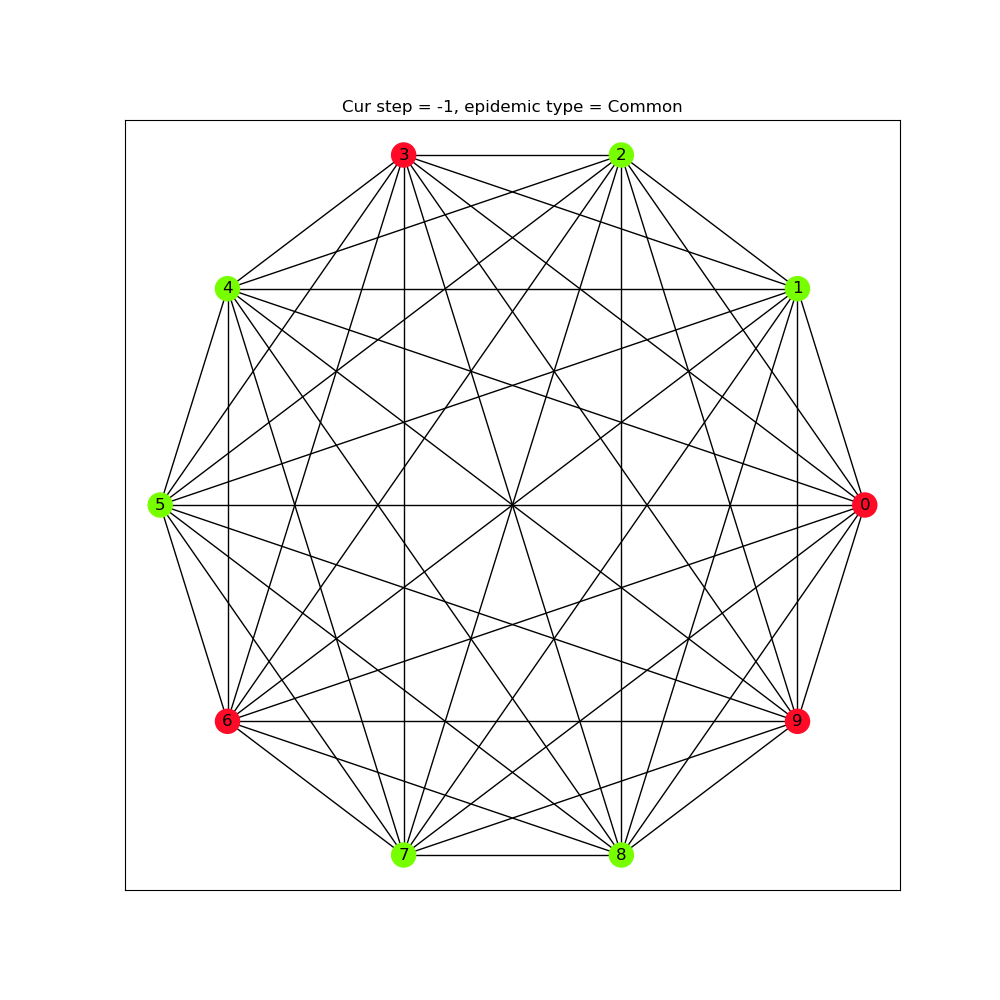
\includegraphics[width=0.32\linewidth, keepaspectratio]{../figs/evidence2/init}}
		\subfigure[Вид <<домашнего>> графа]{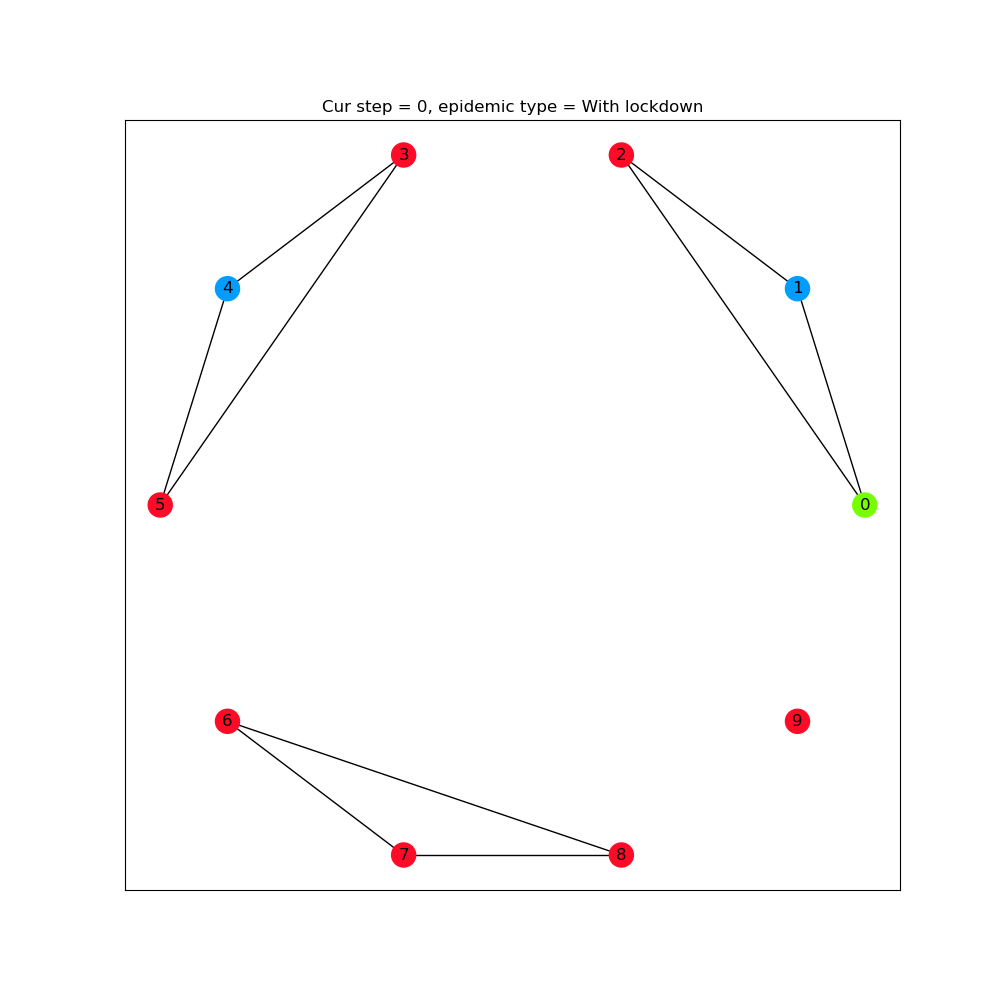
\includegraphics[width=0.32\linewidth, keepaspectratio]{../figs/evidence2/start_with_ld}}
		\subfigure[Сравнительные треки эпидемии с локдауном и без него]{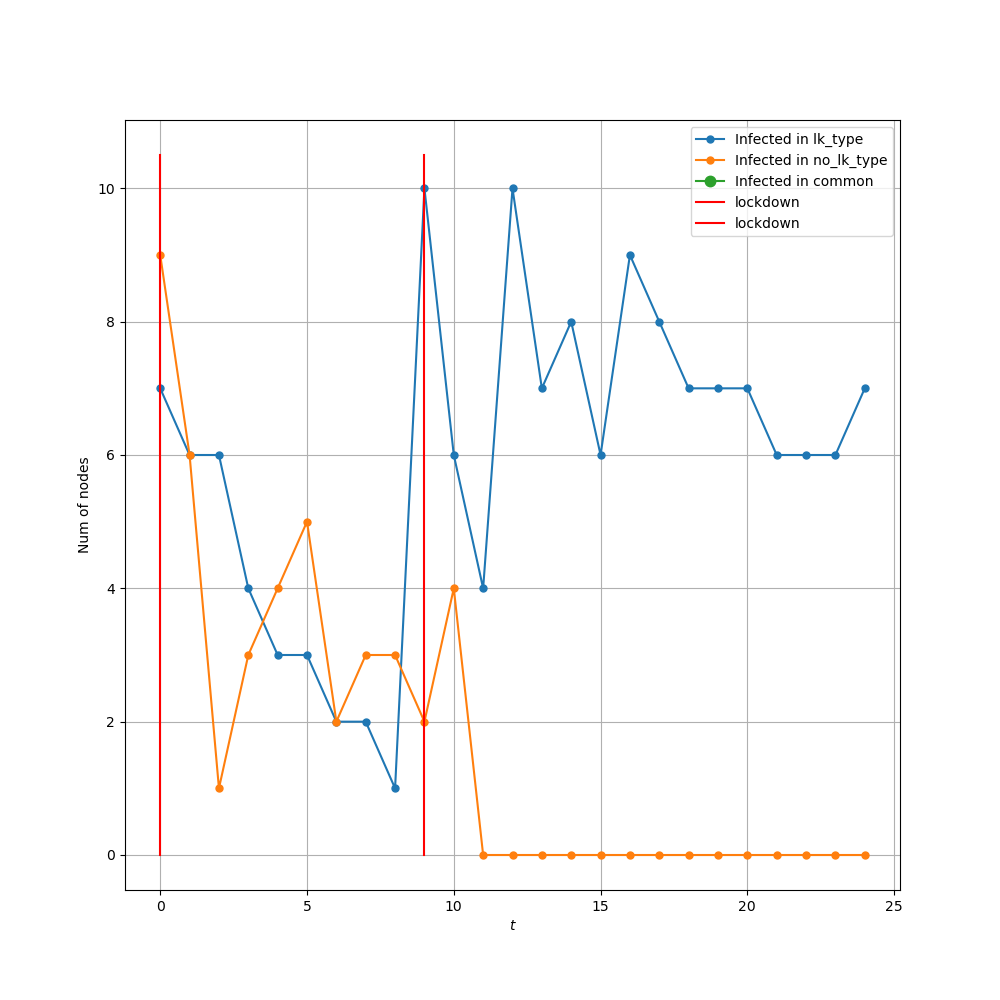
\includegraphics[width=0.32\linewidth, keepaspectratio]{../figs/evidence2/tracks}}
		
	\end{figure}

	\begin{center}
		\textbf{{\large Полный граф}}
	\end{center}
		
	\end{frame}

	\begin{frame}{Эксперимент}
		
		\begin{figure}
			\renewcommand{\thesubfigure}{}
			
			\subfigure[Начальная конфигурация]{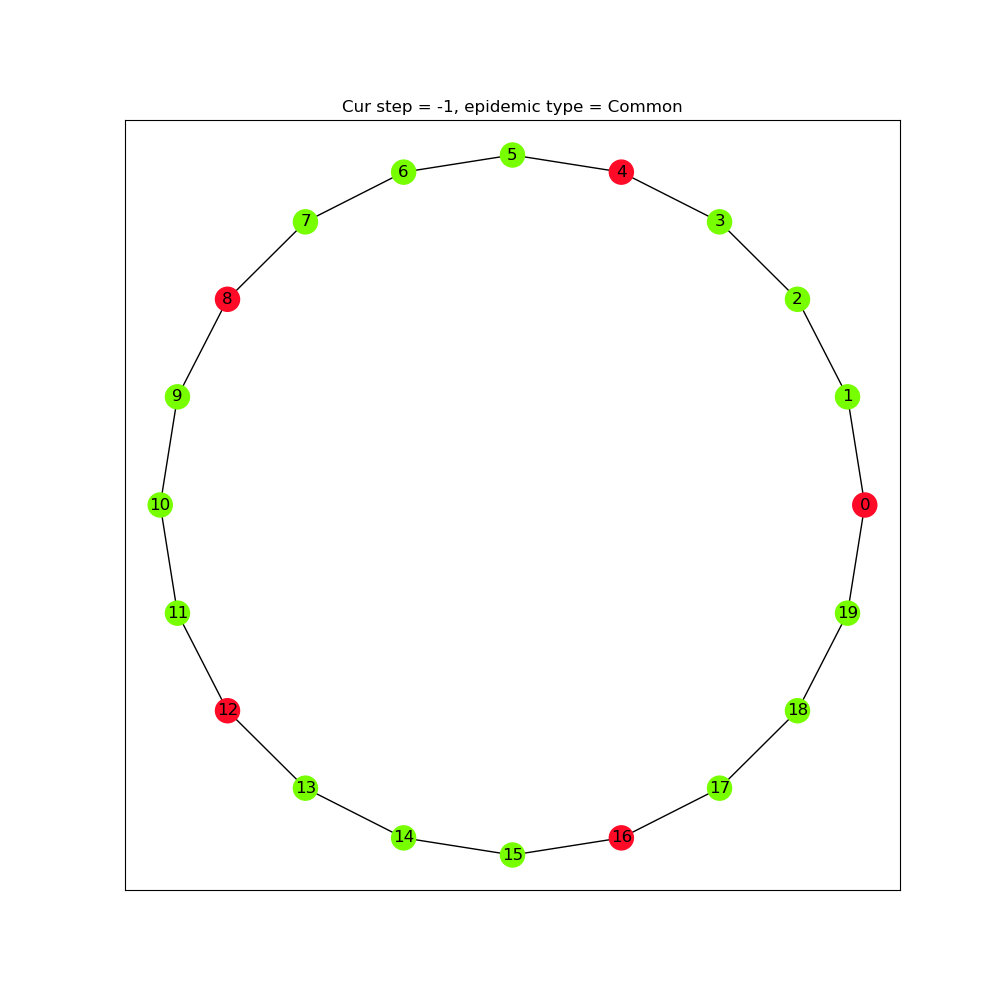
\includegraphics[width=0.32\linewidth, keepaspectratio]{../figs/evidence3/init}}
			\subfigure[Вид <<домашнего>> графа]{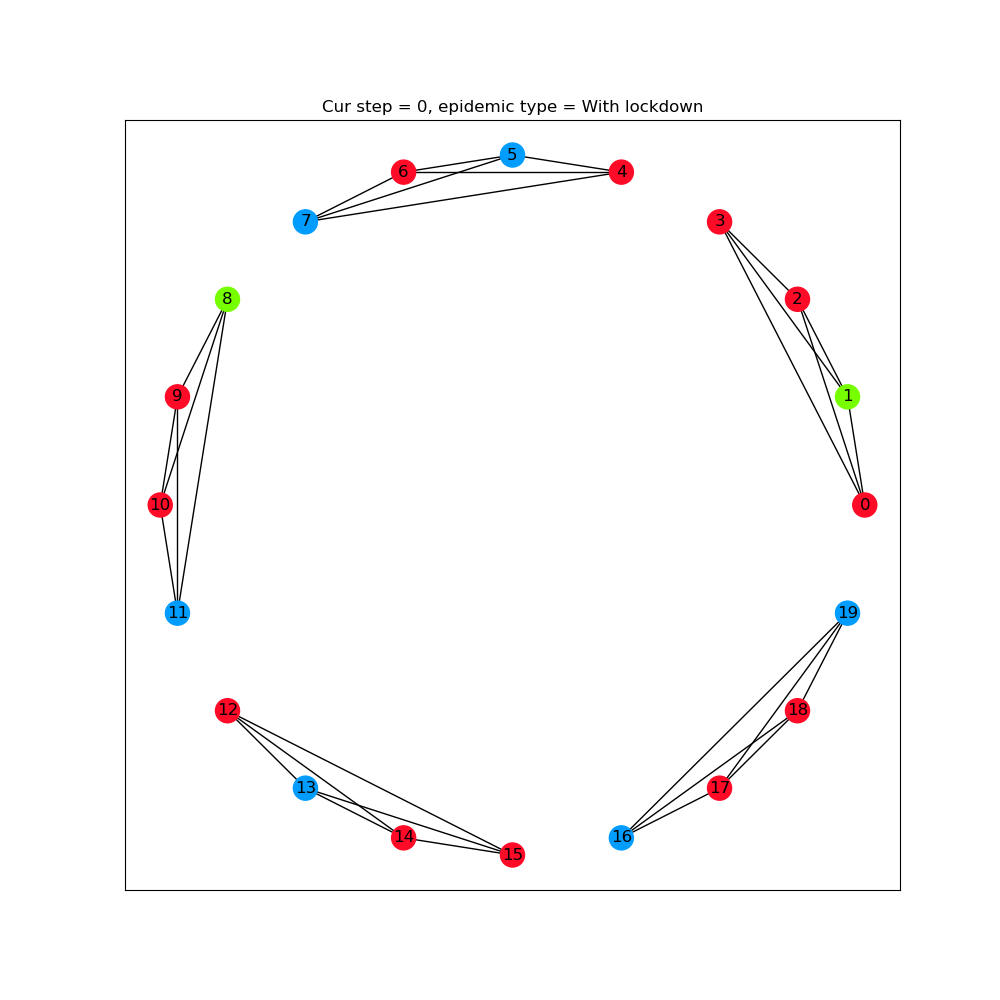
\includegraphics[width=0.32\linewidth, keepaspectratio]{../figs/evidence3/start_with_ld}}
			\subfigure[Сравнительные треки эпидемии с локдауном и без него]{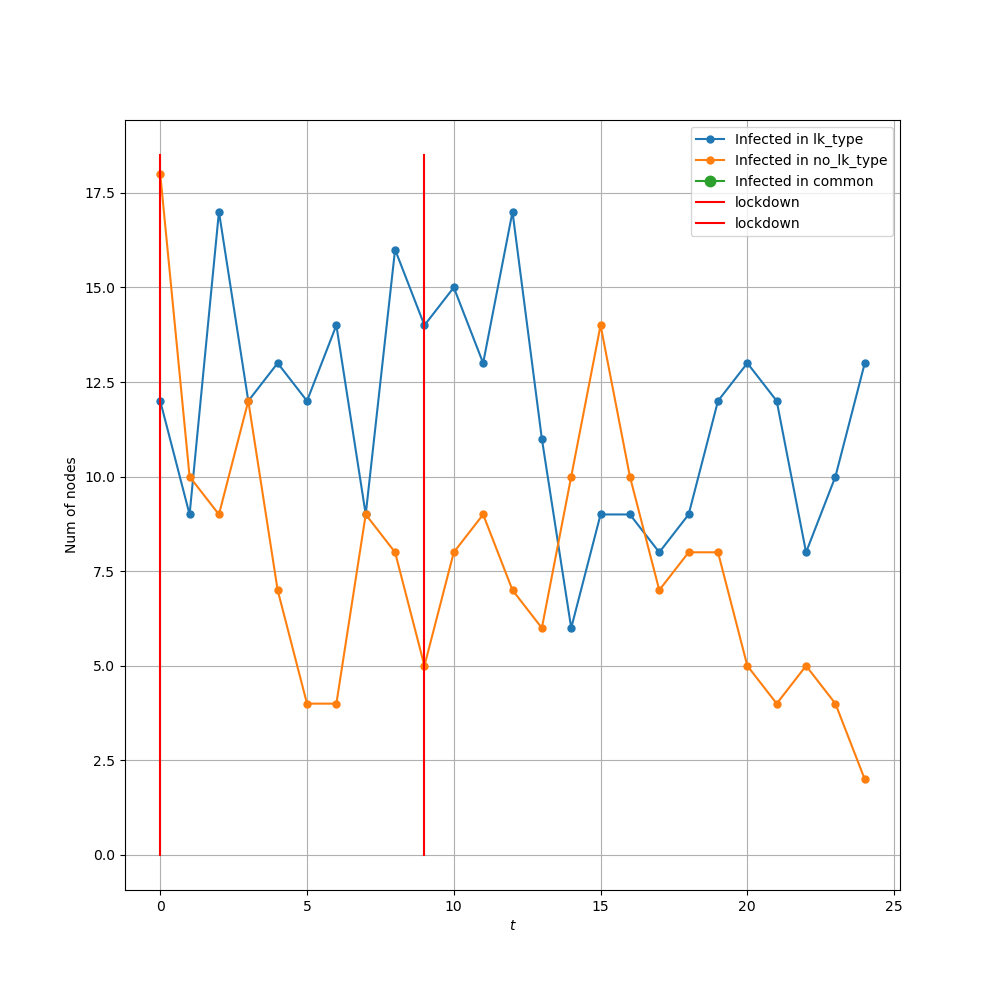
\includegraphics[width=0.32\linewidth, keepaspectratio]{../figs/evidence3/tracks}}
		
		\end{figure}
	
	\begin{center}
		\textbf{{\large Граф-цикл}}
	\end{center}
		
	\end{frame}

	\begin{frame}{Анализ ошибки}
		
	\end{frame}

	\begin{frame}{Заключение}
		
	\end{frame}
	
\end{document}